%%% optionally include ngerman in the document class options list
\documentclass[ngerman, paper=a4, 11pt, cleardoubleempty, twoside, openright, BCOR=7mm, DIV12, idxtotoc, liststotoc, bibtotoc, headinclude=false]{scrreprt}
\usepackage[utf8]{inputenc}

%%% uncomment only one of the following two lines %%%
\usepackage[ngerman]{babel}
% \usepackage[english]{babel}

\usepackage[T1]{fontenc}
\usepackage{format}

\title{Design und Implementierung eines Referenzsystems zur indoor Lokalisierung auf Basis RGB-D Featuretrackings}
\author{Benjamin Aschenbrenner}
\matrikelno{4292264}
\thesis{Bachelorarbeit}
\assistentName{Dipl.-Inf. Heiko Will}

\automark[section]{chapter}
\begin{document}
	%===================================
	% Titlepage
	%===================================
	\pagenumbering{roman}
	\maketitle
	\cleardoublepage
	
	%===================================
	% Official parts
	%===================================
	\affirmation
	\chapter*{\abstractname}
% delete german abstract when writing in english
\section*{Zusammenfassung}
orem ipsum dolor sit amet, consetetur sadipscing elitr, sed diam nonumy eirmod tempor invidunt ut labore et dolore magna aliquyam erat, sed diam voluptua.At vero eos et accusam et justo duo dolores et ea rebum. Stet clita kasd gubergren, no sea takimata sanctus est Lorem ipsum dolor sit amet. Lorem ipsum dolor sit amet, consetetur sadipscing elitr, sed diam nonumy eirmod tempor invidunt ut labore et dolore magna aliquyam erat, sed diam voluptua. At vero eos et accusam et justo duo dolores et ea rebum. Stet clita kasd gubergren, no sea takimata sanctus est Lorem ipsum dolor sit amet. Lorem ipsum dolor sit amet, consetetur sadipscing elitr, sed diam nonumy eirmod tempor invidunt ut labore et dolore magna aliquyam erat, sed diam voluptua. At vero eos et accusam et justo duo dolores et ea rebum. Stet clita kasd gubergren, no sea takimata sanctus est Lorem ipsum dolor sit amet.


% always write an english abstract in addition to a german one
\section*{Abstract}
orem ipsum dolor sit amet, consetetur sadipscing elitr, sed diam nonumy eirmod tempor invidunt ut labore et dolore magna aliquyam erat, sed diam voluptua.At vero eos et accusam et justo duo dolores et ea rebum. Stet clita kasd gubergren, no sea takimata sanctus est Lorem ipsum dolor sit amet. Lorem ipsum dolor sit amet, consetetur sadipscing elitr, sed diam nonumy eirmod tempor invidunt ut labore et dolore magna aliquyam erat, sed diam voluptua. At vero eos et accusam et justo duo dolores et ea rebum. Stet clita kasd gubergren, no sea takimata sanctus est Lorem ipsum dolor sit amet. Lorem ipsum dolor sit amet, consetetur sadipscing elitr, sed diam nonumy eirmod tempor invidunt ut labore et dolore magna aliquyam erat, sed diam voluptua. At vero eos et accusam et justo duo dolores et ea rebum. Stet clita kasd gubergren, no sea takimata sanctus est Lorem ipsum dolor sit amet.


	\cleardoublepage
	
	\tableofcontents
	\listoffigures
	\listoftables
	\lstlistoflistings
	\printglossaries
  \cleardoublepage
  \pagenumbering{arabic}
    
	%===================================
	% Main part of the text
	%===================================	
	\chapter{Einleitung} 
	\label{cha:einleitung}
	\section{Motivation}
\label{sec:motivation}
%==============================================================================

Systeme zur Positionsbestimmung werden für zahlreiche Zwecke genutzt und deren Bedeutung wächst parallel zur
Verbreitung immer neuer sogenannter \textit{location based services} und deren wachsender Nutzung.
Für Anwendungen im Freien haben sich satelliten gestütze Systeme, welche hohe Genauigkeit bieten, etabliert.
Als bekanntes Beispiel sei hier das \textit{NAVSTAR-GPS} genannt, welches sich auch zivil nutzen lässt.
Allerdings ergeben sich viele Anwendungsumgebungen, in denen derartige Systeme gar nicht, bzw.
nur ungenau funktionieren oder bewusst aus Kostengründen gemieden werden. 
Dies sind typischerweise Umgebungen in denen die Sattelitensignale zu stark gedämpft werden oder
vorallem durch Reflexionen bedingte Laufzeitverschiebungen, sich negativ auf die Genauigkeit auswirken, wie z.B.: 

%Eventuell wird auch aus Kostengründen auf einen GPS Empfänger verzichtet.
%mehr Quellen anbringen !!
%(Aufzählen: innerhalb von Gebäuden, Untergrund...(Signalabschirmung), ungenau Mehrwegausbreitung in urbanen Umgebungen)

\begin{itemize}
  \item innerhalb von Gebäuden (``indoor'')
  \item im Untergrund (Tunnel, Höhlen u.ä.)
  \item im Bereich dicht bebauter urbaner Gebiete (Mehrwegausbreitung)
\end{itemize}

Um in solchen Umgebungen dennoch Lokalisierung zu ermöglichen wurden und werden viele theoretische Konzepte und 
konkrete Systeme entwickelt. Einen Überblick hierzu bietet
Quelle anbringen (mobile entity localization and tracking in GPS less enviroments - Buch)
Auch in der Arbeitsgruppe \textit{Computer Systems & Telematics}, an der \textit{FU-Berlin}, 
wurde dem Problem der indoor Lokalisierung mit der Entwicklung eines \textit{Wireless Sensor Network (WSN)}
basiertem Systems im Rahmen des Forschungsprojektes \textit{FeuerWhere}, begegnet. 
Dieses Projekt entstand u.a. in Kooperation mit der Berliner Feuerwehr.
Ziel bei der Entwicklung war ein flexibles indoor Lokalisierungssystem zu schaffen, welches mit
low-cost Komponenten aufgebaut wird. 
Im Kern ist das System in der Lage die Entfernung zwischen den involvierten Sensorknoten zu bestimmen und 
dadurch Rückschlüsse auf die Position zu gewinnen.

-kurz halten:
-Signallaufzeitmessung
-zwei Arten von Knoten feste anchor Knoten mit bekannter Postion 
-restliche Knoten sind mobil
-Positionsbestimmung?

-Notwendigkeit zum Test weil:
  -Laufzeitmessung fehlerbehaftet
  -Mehrwegausbreitung indoor
  -viele Stellschrauben der Positionsbestimmung


	\section{Lösungsansätze}
\label{sec:loesungsansaetze}
%==============================================================================
lorem ipsum!
	\section{Aufgabenstellung}
\label{sec:aufgabenstellung}
%==============================================================================
TODO

\begin{itemize}
  \item allgemeines Ziel formulieren
    \begin{enumerate}
      \item mobiles Testsystem
      \item Steuerung (autonom/Tastatur)
      \item Aufzeichnen des Pfades
      \item Karte erstellen und Pfad dort einzeichnen
    \end{enumerate}
\end{itemize}



	\chapter{Umsetzung} 
	\label{cha:umsetzung}
	\section{Konzept}
\label{sec:konzept}
%==============================================================================
lorem ipsum!
	\section{Soft- und Hardware}
\label{sec:softundhardware}
%==============================================================================

Im Folgenden werden die wichtigsten Konzepte näher erläutert.

\subsection{Microsoft Kinect}
\label{subsec:kinect}

Microsoft bietet seit November 2010 {\color{red}Quelle} ein Produkt an, das es in dieser günstigen Form zuvor nicht auf dem Markt gab: die \gls{glos:Kinect}. Die Designgrundlage stammt von einer Firma namens PrimeSense\footnote{siehe \url{http://www.primesense.com/}}, die schon seit geraumer Zeit derartige Geräte entwickelt. Eigentlich wurde das Gerät für Microsofts \gls{glos:XBOX} konzipiert, jedoch wuchs das Interesse daran stetig, als Open Source Projekte entstanden die das Protokoll über die USB-Schnittstelle zur \gls{glos:Kinect} per \gls{glos:RevEng} offenlegten. Heute wird sie in unzähligen Hobby- aber auch professionellen zu einem großen Teil universitären Projekten wie diesem eingesetzt. Dabei inspirierten die Entwickler zunächst vor allem Anwendungen bezüglich Gestensteuerung oder Skeleton Tracking wie sie auch in den Konsolenspielen eingesetzt werden. Jedoch wurde schnell ersichtlich, das das Gerät aufgrund seiner Daten in bestimmten Anwendungsfällen auch Laserscanner ersetzen und damit viele Anwendungsszenarien bedienen kann.

{\color{red}fakten:}\\

{\color{red}- aufbau (kamera, ir, ir-kamera)}\\
{\color{red}- Auflösung}\\

Die \gls{glos:Kinect} sendet über den {\color{red}AUSFÜLLEN} ein Muster aus Infrarotpunkten aus. Wie in Abbildung \ref{fig:kinectIlluminator} zu sehen, werden diese von Objekten die im Sichtfeld des Gerätes stehen reflektiert. Gut zu erkennen ist auch, dass sich in der Szene eine flache Grundfläche und zwei senkrecht aneinander stehende leicht konvexe Flächen befinden. Aufgrund dieses Szenenaufbaus, entsteht eine ungleichmäßige Infrarotausleuchtung. Eine spezielle Software kann nun anhand der Verzerrung des Musters, dem Abstand und Größe der Infrarotlichtpunkte errechnen, in welcher Entfernung die Objekte zur Kamera stehen.
\begin{figure}[t]
	\centering
	\fbox{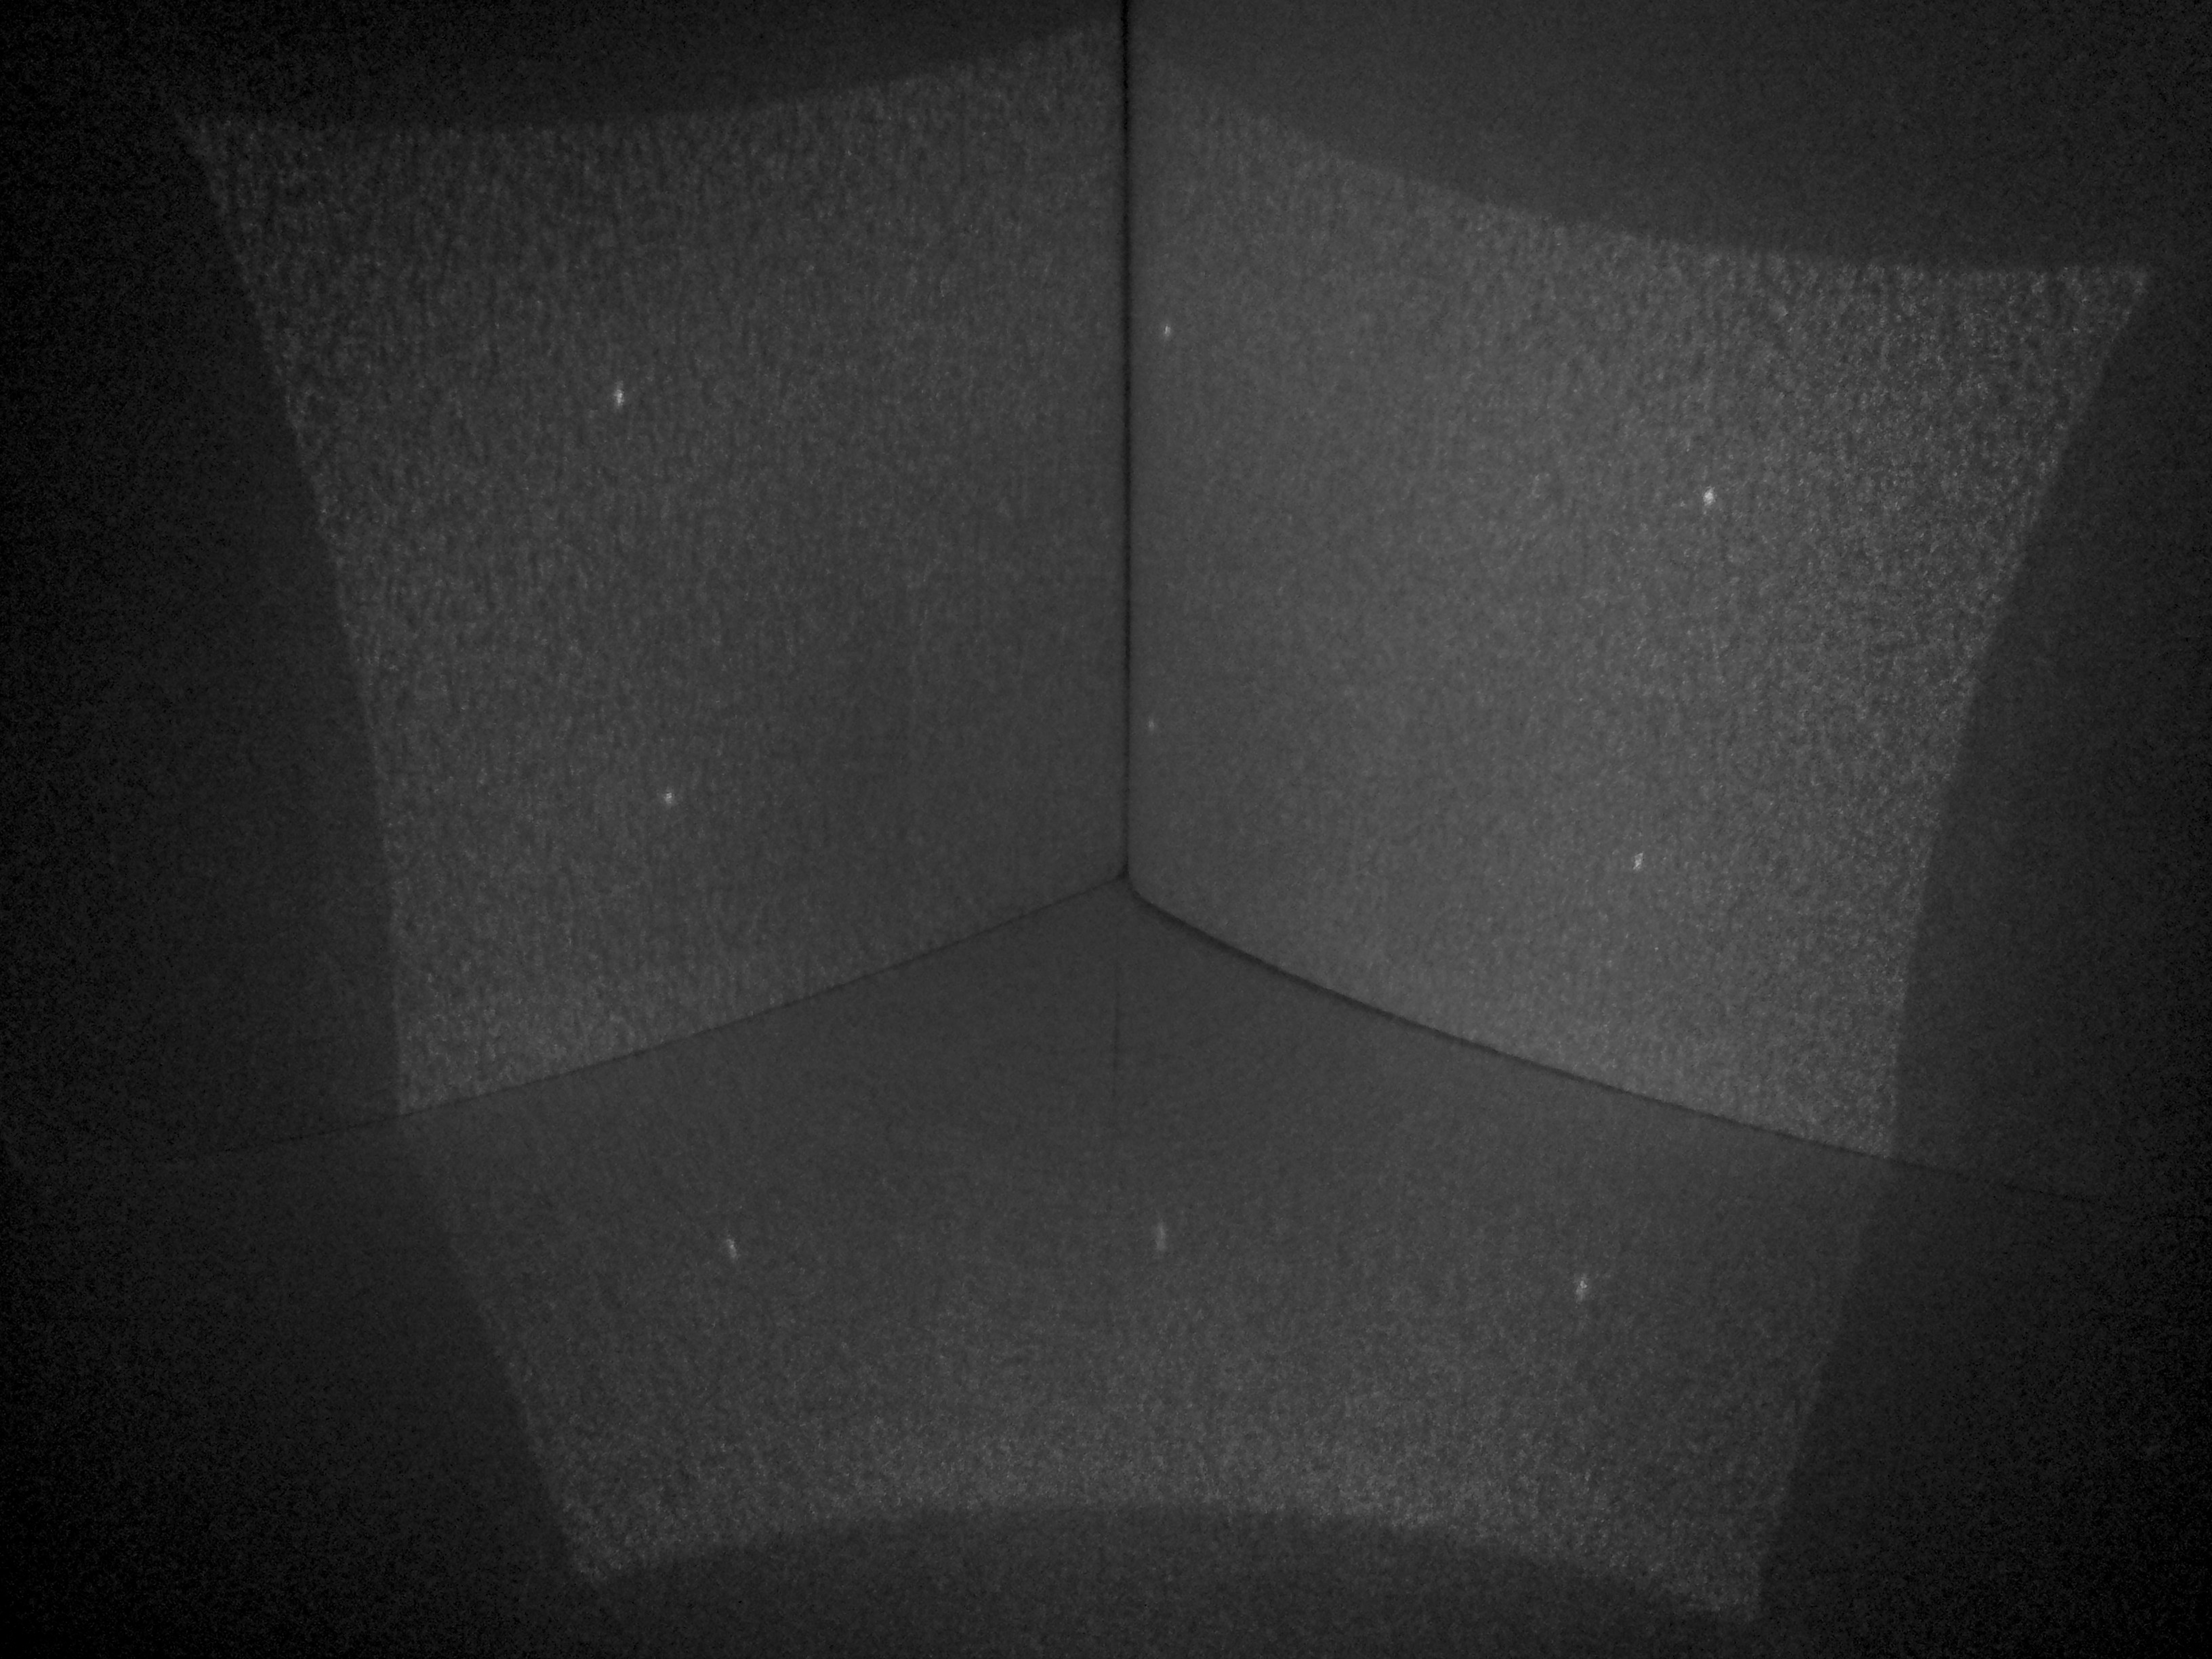
\includegraphics[height=10cm]{./graphics/kinectIlluminator_sharp2}}
	\caption[Kinect Infrarot Feld]{Eine Aufnahme des Infrarot Ausleuchtungsfelds der \gls{glos:Kinect}.}
	\label{fig:kinectIlluminator}
\end{figure}

Aufgrund des Aufbaus der \gls{glos:Kinect} entstehen dabei zwangsläufig tote Winkel, über die sie keine Aussagen treffen kann. Abbildung \ref{fig:toterWinkel} zeigt diesen Umstand. Das Infrarotlicht kann nicht auf die ganze hintere Wand projiziert werden, da diese von einem davor stehenden Objekt verdeckt wird. Der {\color{red}rote} Bereich liegt jedoch im Sichtfeld der Infrarotkamera. Die Abbildung \ref{fig:kinectViews} in Kapitel \ref{subsec:opennistack} zeigt diesen Effekt ebenfalls. Jedoch ist dort der Winkel des linken 3D-Bildes leicht verschoben, sodass tote Winkel scheinbar links und rechts von Objekten auftreten können. Dies ist aber wie in Abbildung \ref{fig:toterWinkel} gezeigt aufgrund des Aufbaus der \gls{glos:Kinect} nicht der Fall.
\begin{figure}[t]
	\centering
	\fbox{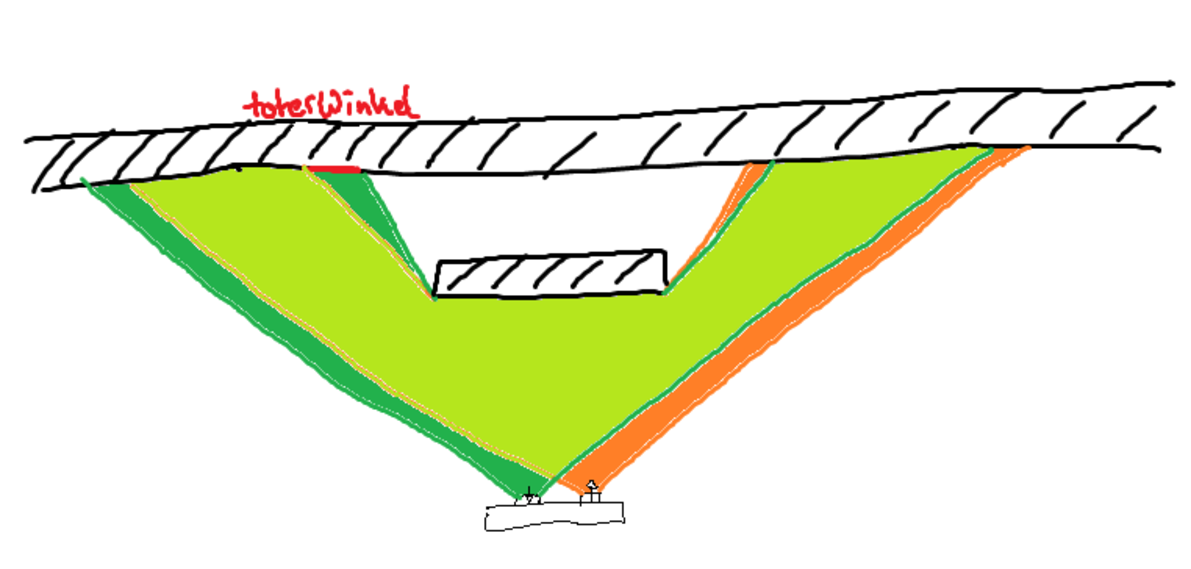
\includegraphics[height=6cm]{./graphics/toterWinkel}}
	\caption[Toter Winkel der Kinect]{Eine anschauliche Darstellung eines toten Winkels der \gls{glos:Kinect}.}
	\label{fig:toterWinkel}
\end{figure}

{\color{red}- Reichweite}\\
{\color{red}- Genauigkeit in Abhängigkeit zur Entfernung (kurvenbild: kinect/optimal-linien)}\\
{\color{red}- vergleich mit laser (kinect ca. 80 EUR, laser ca. 1500 EUR)}\\

{\color{red}
benutzungsmöglichkeiten für uns:\\
- libfreenect, (inoffizielle api)\\
- openni (offizielle api)\\
- openni\_kinect stack erwähnen/referenzieren! (benutzt offizielle api)\\
}

Die beiden erwähnten Bibliotheken funktionieren zwar gut, jedoch ist ein großer Aufwand von Nöten um diese Daten in verwendbare Strukturen zu bringen. Es wurde bereits von verschiedenen Universitäten und Forschungseinrichtungen {\color{red}Forschung} betrieben, die sich mit derartigen Daten und deren sinnvoller und effizienter Verwendung auseinandergesetzt hat. Daher liegt es nahe, daraus resultierende quelloffene Software zu benutzen. Im Laufe der Vorbereitung dieser Arbeit wurden zwei solche Software Frameworks evaluiert, die beide Treiber für die Kinect beinhalten: Das \gls{MRPT} beschrieben in \cite{online:mrpt} und \gls{ROS}. \gls{MRPT}, hauptsächlich von der Universidad de Málaga (Spanien) seit 2005\footnote{siehe \cite{online:mrptentwickler}} entwickelt, liefert einige \gls{SLAM} Algorithmen, kann aber nicht mit \gls{ROS} bezüglich der Ortsabstraktion durch die Kommunikationsinfrastruktur konkurrieren. Auch existiert bei \gls{ROS} eine sehr viel größere Entwicklergemeinde. \gls{MRPT} legt vor allem einen großen Wert auf Kapselung verschiedener Algorithmen, während \gls{ROS} auf die Kapselung von Funktionalitäten achtet. Dadurch kann der Anwender eine getestete Funktionalität benutzen, ohne im Detail die verwendeten Algorithmen evaluieren zu müssen. Auch bietet \gls{ROS} bereits Möglichkeiten Roboter zu steuern, und diese Steuerung mit den Funktionalitäten direkt zu verknüpfen und arbeiten zu lassen, da die Schnittstellen zwischen diesen per Design gegeben sind. Zudem existiert in \gls{ROS} ein Tool namens \emph{rviz}, welches im nächsten Kapitel näher erläutert wird. Dieses sorgt dafür, dass Informationen, die innerhalb des Frameworks ausgetauscht werden, visualisiert werden können. Da \gls{MRPT} und auch andere dies im Moment noch nicht bieten können, wurde \gls{ROS} als Grundlage für das Referenzsystem gewählt. Im nächsten Abschnitt wird \gls{ROS} vorgestellt und die wichtigsten Konzepte näher erläutert.

\subsection{Robot Operating System}

{\color{red}Willow Garage erwähnen (seit wann entwickelt?)}

\gls{ROS} ist ein Open-Source Betriebssystem, welches viele Probleme und Aspekte verteilter, komplexer Software bezüglich der Anwendungsentwicklung für Roboter kapselt. Falls nicht anders gekennzeichnet, dient \cite{Quigley:2009kx} in diesem Abschnitt als Quelle.

Im eigentlichen Sinne ist \gls{ROS} kein Betriebssystem. Vielmehr handelt es sich um ein leichtgewichtiges C++ Framework, das in einem bestehenden Betriebssystem ausgeführt wird. Dabei verwendet es eine Peer-to-peer Kommunikationsarchitekur, mit Hilfe derer einzelne Programme in verschiedenen Programmiersprachen unabhängig voneinander kommunizieren können. \gls{ROS} legt zudem großen Wert auf eine Tool-basierte Funktionsweise. Das heißt, dass alles strikt in Module gegliedert ist, wodurch das Framework selbst sowie die einzelnen Module besonders gut getestet werden können.

In dieser Arbeit dient \gls{ROS} als eine robuste Architektur zum Transport verschiedener Daten zwischen Programmen, die bei Bedarf auch auf verschiedenen Computern im Netzwerk ausgeführt werden können. Wie in den Kapiteln \ref{sec:pathfinder} und \ref{sec:navstack} näher beschrieben, bietet \gls{ROS} bereits einen großen Funktionsumfang bezüglich des Umgangs mit Robotern. Im Folgenden wird eine kurze Einführung in die generelle Architektur sowie in in dieser Arbeit benötigte Tools gegeben.

\subsubsection{Architektur}

Einzelne Module beziehungsweise Programme in einer \gls{ROS} Umgebung werden \glspl{glos:Node} bezeichnet. Diese können beliebg oft unter Angabe eines Namensraumes gestartet werden. Das heißt ein \gls{glos:Node} kann generisch Aufgaben lösen, ohne zu wissen, ob er beispielsweise gerade den rechten oder linken Arm eines Roboters repräsentiert.

Damit ein \gls{glos:Node} unter \gls{ROS} übersetzt beziehungsweise ausgeführt werden kann, muss er einem \gls{glos:Package} zugeordnet sein. Ein \gls{glos:Package} kann mehrere \glspl{glos:Node} beinhalten. Es definiert durch eine \gls{glos:Manifest} Datei, welche Abhängigkeiten es zu anderen \glspl{glos:Package} besitzt. Mehrere \glspl{glos:Package} können zu einem \gls{glos:Stack} zusammengeschlossen sein, beispielsweise wenn sie eine gemeinsame Aufgabe erfüllen, indem sie diese in Teilaspekte zerlegen. Ein solcher \gls{glos:Stack} besitzt dann ebenfalls ein \gls{glos:Manifest}.

Innerhalb der \glspl{glos:Package} oder \glspl{glos:Stack} können \glspl{glos:LaunchFile} angelegt werden, die das Starten eines ganzen Systems mit mehreren \glspl{glos:Node} erleichtern. Dabei kann in einer solchen Datei auch definiert sein, dass bestimmte \glspl{glos:Node} nicht lokal, sondern entfernt auf einem anderen Computer gestartet werden. Außerdem können hier Parameter an die \glspl{glos:Node} übergeben werden, die sich üblicherweise nur selten ändern. \glspl{glos:LaunchFile} können zudem andere \glspl{glos:LaunchFile} rekursiv inkludieren und dabei auch Parameter überschreiben{\color{red} (Inernet-)Quelle dafür angeben, da nicht in angegebener Quelle)}. Verzichtet man auf eine \gls{glos:LaunchFile}, dann müssen die \glspl{glos:Node} einzeln gestartet und auch wieder beendet werden. Durch die \gls{glos:LaunchFile} können alle gestarteten \glspl{glos:Node} über STRG+C zusammen beendet werden.

\glspl{glos:Node} kommunizieren über das \gls{ROS} interne Kommunikationsnetzwerk miteinander. Das heißt, wenn ein \gls{glos:Node} Informationen anderen \glspl{glos:Node} zur Verfügung stellt, veröffentlicht er diese über ein bestimmtes \gls{glos:Topic}. Andere \glspl{glos:Node} können dieses \gls{glos:Topic} abonnieren. Dabei haben \glspl{glos:Topic} immer einen bestimmten Namen, der sowohl durch \glspl{glos:Node}, die Informationen veröffentlichen, als auch von \glspl{glos:Node} die Informationen abonnieren, die sie benötigen um ihre Funktionalität zu erfüllen, festgelegt sein kann. Um einen Konflikt zu vermeiden, muss in einem konkreten System in der \gls{glos:LaunchFile} eine Abbildung zwischen \gls{glos:Topic} Benennungen stattfinden. \glspl{glos:Node} können zudem sehen, ob ihr eigenes \gls{glos:Topic} abonniert wurde. Dadurch lässt sich Rechenzeit sparen, sollte kein Abonnent vorhanden sein.

Informationen werden in \glspl{glos:Message} zu einem \gls{glos:Topic} veröffentlicht. Sie werden zunächst in einer platformunabhängigen Sprache definiert, einer \gls{IDL}. Diese Abstraktion erlaubt es, in wenigen Zeilen eine \gls{glos:Message} zu definieren. Entsprechende Code Generatoren in verschiedenen Sprachen erzeugen automatisch aus dieser Definition Klassen, welche durchaus hunderte Zeilen Code umfassen können. Dadurch fällt es dem Programmierer sehr viel einfacher, in \gls{ROS} sprachenunabhängig neue zuvor nicht bekannte \glspl{glos:Message} zu definieren. Viele oft benötigte \glspl{glos:Message} werden beispielsweise bereits durch den \emph{common\_msgs} \gls{glos:Stack} zur Verfügung gestellt. Zusätzlich zur \gls{glos:Topic} Architektur gibt es in \gls{ROS} \glspl{glos:Service}, welche einen optionalen Parameter erhalten, und üblicherweise einen Rückgabewert liefern. Durch diese kann eine synchrone Kommunikation zwischen \glspl{glos:Node} stattfinden. 

\subsubsection{Tools}

{\color{red}Quellen finden!}

Ein \gls{glos:Package} wird über das Tool \emph{rosmake PACKAGE\_NAME} kompiliert. Dabei werden falls nötig alle Abhängigkeiten die in der \gls{glos:Manifest} Datei eingetragen wurden ebenfalls rekursiv kompiliert. Ein \gls{glos:Package} mit mehreren \glspl{glos:Node} besitzt somit mehrere ausführbare Dateien, die über \emph{rosrun PACKAGE\_NAME NODE\_NAME} einzeln, über \emph{roslaunch PACKAGE\_NAME LAUNCH\_DATEI\_NAME} zusammen, gestartet werden.

Damit gestartete \glspl{glos:Node} sich in \gls{ROS} finden, gibt es einen Namensdienst, den sogenannten Master. Alle \glspl{glos:Node} melden sich an diesem Dienst an, und erhalten hierüber Direktverbindungen zu anderen \glspl{glos:Node}. Dieser Dienst wird entweder über die Konsole mit dem Befehl \emph{roscore}, oder implizit durch Benutzung einer \gls{glos:LaunchFile} gestartet. Ein spezieller \gls{glos:Node} namens \emph{rosout} wird immer gemeinsam mit dem Master gestartet. Er bekommt automatisch Log Nachrichten aller \glspl{glos:Node}. Diese können an zentraler Stelle mit dem Tool \emph{rxconsole} angezeigt werden.

Da eine Topographie mit vielen \glspl{glos:Node} sehr unübersichtlich sein kann, bietet \gls{ROS} ein Tool namens \emph{rxgraph} an. Dieses Tool zeigt alle \glspl{glos:Node} visuell als Knoten und verbindet diese, sollten sie \glspl{glos:Topic} einander abonnieren.

Um einzelne \glspl{glos:Node} oder ein ganzes System zu testen, kann es sinnvoll sein, bestimmte Daten beispielsweise einer Kamera oder eines Roboters, bei einem normalen Test aufzunehmen und anschließend so wieder abzuspielen, dass der eigene noch zu entwickelnde \gls{glos:Node} mit diesen Daten als Eingabe getestet werden kann. \gls{ROS} stellt hierfür das Tool \emph{rosbag} zur Verfügung. Mittels \emph{rosbag record TOPIC\_NAME(N) -O DATEI} werden ein oder mehrere \glspl{glos:Topic} abonniert und in einer einzelnen Datei aufgezeichnet. Über \emph{rosbag play DATEI(-EN)} werden eventuell mehrere solche Dateien gleichzeitig wieder abgespielt. Dabei werden die Zeitstempel beachtet, die in einer jeden aufgezeichneten \gls{glos:Message} enthalten sind. Die Reihenfolge, in der die \glspl{glos:Message} während des Aufzeichnens erstellt wurden, entspricht also auch der Abspielreihenfolge.

\glspl{glos:Message} transportieren üblicherweise Daten, die visualisiert werden können. \gls{ROS} hält hierfür einen \gls{glos:Node} namens \gls{glos:rviz} bereit. Dieser versteht bereits einige \glspl{glos:Message}, kann aber auch bei Bedarf durch Plug-Ins erweitert werden. In dieser Arbeit wird \gls{glos:rviz} beispielsweise dafür eingesetzt, eine Karte und einen Roboter darin anzuzeigen. Hierbei wird deutlich, dass \gls{glos:rviz} die Transformation zwischen Karte und Roboter kennen muss. Dafür sorgt ein sehr wichtiges \gls{glos:Package} namens \emph{tf}. Jede \gls{glos:Message} ist in einem bestimmten Koordinatensystem entstanden, einem sogenannten \gls{glos:CFrame}, welcher in einer \gls{glos:Message} durch einen String repräsentiert wird. Der \emph{tf}-\gls{glos:Node} abonniert nun alle \emph{tf-\glspl{glos:Message}}, die zu einem \gls{glos:Topic} namens \emph{/tf} beispielsweise von Sensoren veröffentlicht werden. Andere \glspl{glos:Node}, die die Transformation zwischen zwei \glspl{Frame} benötigen, wie beispielsweise \gls{glos:rviz} zum Visualisieren der \glspl{glos:Message}, können nun anhand der gesammelten Daten des \emph{tf-\glspl{glos:Node}} diese direkt ablesen. Diese Transformationen werden in einer Baumstruktur vorgehalten. Es muss also zwischen zwei \glspl{Frame} immer genau eine Hierarchie geben. In \gls{glos:rviz} selbst, kann der Anwender einen globalen \gls{glos:FFrame} wählen, in den alle sonstigen \glspl{Frame} unter Beachtung ihrer Transformation zu diesem gezeichnet werden, typischerweise also die Wurzel des \emph{tf}-Baumes. Zusätzlich lässt sich ein \gls{glos:TFrame} auswählen, den der Benutzer verfolgen möchte. Wird also eine Karte als \gls{glos:TFrame} gewählt, bewegt sich der Roboter. Wird der Roboter selbst ausgewählt, bewegt sich die Karte während der Roboter immer in der Mitte bleibt.

\subsection{OpenNI\_Kinect Stack}
\label{subsec:opennistack}

Der OpenNI\_Kinect Stack integriert unter Anderem die in \ref{subsec:kinect} beschriebene Kinect in \gls{ROS}. Er erlaubt neben Skeleton Tracking und Gesture Recognition auch die direkte Verwendung der Rohdaten der \gls{glos:Kinect} durch das \gls{glos:Package} \emph{openni\_camera}. Wie in \cite{online:rosopenni_camera} beschrieben, werden durch das Starten des \emph{openni\_camera} \glspl{glos:Node} u. a. die in der Tabelle \ref{tab:opennicameramsgs} {\color{red} (steht hier immer noch ein doppeltes fragezeichen?)} beschriebenen \glspl{glos:Message} zu den jeweiligen \glspl{glos:Topic} veröffentlicht.
\begin{table}
\label{tab:opennicameramsgs}
\begin{tabular}{ l l p{4.3cm} }
	\hline
	\gls{glos:Message}			&	\gls{glos:Topic}						& 	Beschreibung\\
	\hline
	sensor\_msgs/CameraInfo		&	/camera/depth/camera\_info			&	Parameter der Infrarot Kamera\\
	stereo\_msgs/DisparityImage	&	/camera/depth/disparity				&	{\color{red}was ist das, brauchen wir das?}\\
	sensor\_msgs/Image			&	/camera/depth/image					&	Tiefenbild, enthält die Entfernungen in Metern\\
	%sensor\_msgs/CompressedImage	&	/camera/depth/image/compressed		&	\\
	%sensor\_msgs/Image			&	/camera/depth/image\_raw				&	\\
	%sensor\_msgs/CompressedImage	&	/camera/depth/image\_raw/compressed	&	\\
	sensor\_msgs/PointCloud2		&	/camera/depth/points					&	farblose \gls{glos:Pointcloud}\\
	\hline
	sensor\_msgs/CameraInfo		&	/camera/rgb/camera\_info				&	Paramter der RGB Kamera\\
	sensor\_msgs/Image			&	/camera/rgb/image\_color				&	RGB Bild\\
	%sensor\_msgs/CompressedImage	&	/camera/rgb/image\_color/compressed	&	\\
	sensor\_msgs/Image			&	/camera/rgb/image\_mono				&	Bild in Graustufen\\
	%sensor\_msgs/CompressedImage	&	/camera/rgb/image\_mono/compressed	&	\\
	%sensor\_msgs/Image			&	/camera/rgb/image\_raw				&	\\
	%sensor\_msgs/CompressedImage	&	/camera/rgb/image\_raw/compressed		&	\\
	sensor\_msgs/PointCloud2		&	/camera/rgb/points					&	farbige \gls{glos:Pointcloud}\\
	\hline
\end{tabular}
\caption[Topic-Übersicht von openni\_camera]{Übersicht der veröffentlichten Informationen von \emph{openni\_camera}.}
\end{table}
Über jeweils einen \gls{glos:Service} \emph{set\_camera\_info} erlaubt das \gls{glos:Package} zusätzlich eine Konfiguration und Kalibrierung der Infrarot und RGB Kamera.

Eine \gls{glos:Message} des Typs \emph{PointCloud2} wird hier dazu verwendet, 3D Informationen, wie in \cite{online:pointcloud2} näher beschrieben, u.a. durch folgende Komponenten zu veröffentlichen:

\begin{description}
	\item[Header]		Sequenznummer, Zeitstempel und Informationen über den \gls{glos:CFrame}
	\item[Fields]		Liste aller Felder eines Punktes
	\item[Row\_Step]	Länge einer Zeile
	\item[Data]		Liste aller Punkte
\end{description}

In Abbildung \ref{fig:kinectViews} sind zwei solche \glspl{glos:Pointcloud} aus zwei verschiedenen Winkeln dargestellt. Auf der linken Seite ist nahezu die Sicht der \gls{glos:Kinect} zu sehen, während auf der rechten Seite der Sichtwinkel auf die Wolke stark geändert wurde. Beide Bilder wurden zu unterschiedlichen Zeiten aufgenommen, ohne die Position der \gls{glos:Kinect} zu verändern. Dadurch ist ein unterschiedliches Rauschen an den Rändern der Farbbereiche gut zu erkennen. Die Farben wurden entsprechend der Tiefeninformation aus Sicht der \gls{glos:Kinect} gewählt. Dabei wurden nahe Gegenstände mit einer warmen, und entferntere mit kälter werdenden Farben belegt.

\begin{figure}[t]
	\centering
	\fbox{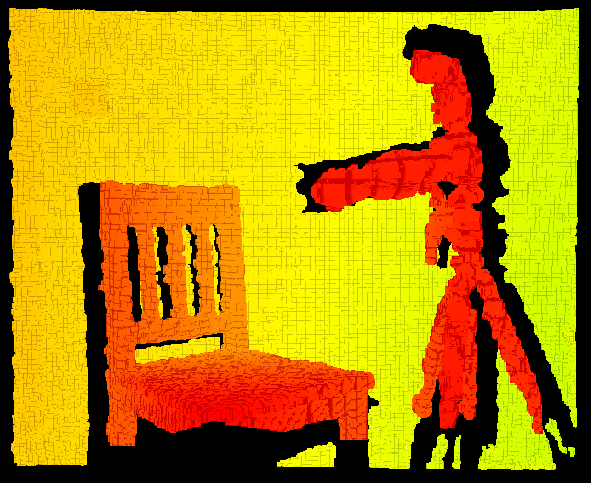
\includegraphics[height=6.5cm]{./graphics/kinectFrontView}}
	\fbox{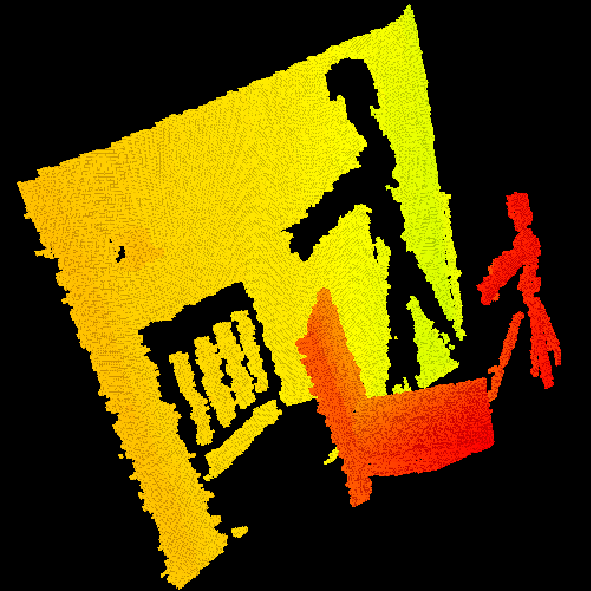
\includegraphics[height=6.5cm]{./graphics/kinectSideView}}
	\caption[Kinect Pointcloud]{Zwei \glspl{glos:Pointcloud} der \gls{glos:Kinect}, visualisiert durch \gls{glos:rviz}.}
	\label{fig:kinectViews}
\end{figure}

\subsection{Turtle Bot}
{\color{red}lorem ipsum!}
	\section{Pathfinder}
\label{sec:pathfinder}
%==============================================================================
{\color{red}lorem ipsum!}

	\chapter{Analyse} 
	\label{cha:analyse}
	\section{Testlauf}
\label{sec:testlauf}
%==============================================================================
lorem ipsum!
	\section{Genauigkeit}
\label{sec:genauigkeit}
%==============================================================================
lorem ipsum!
	\section{Fazit}
\label{sec:fazit}
%==============================================================================
lorem ipsum!

	\chapter{Ausblick} 
	\label{cha:ausblick}
	{\color{red}lorem ipsum!}

	\chapter{Anhang}
	\label{cha:anhang}
	{\color{red}lorem ipsum!}

 %   \chapter{The CST Template}

\section{How to use this Template}
\label{secHowTo}
%==============================================================================
The \gls{CST} thesis template has to be used for all theses of the \gls{DES} sub-research group.
You have to follow some simple rules:
\begin{enumerate}
    \item Use \gls{pdflatex} to compile the \LaTeX\ source code
	\item Do not add files to the repository that are dynamically created by the compiler, e.g., \texttt{*.aux} or the ouput PDF file
	\item Use the \texttt{global-ignores} feature in your \textit{Subversion} configuration file to avoid unintentional uploads, e.g., \\ \texttt{global-ignores = *.aux}
	\item Your report has to be compilable at all times; do not forget to add and upload new files
	\item When removing, moving, or adding files use a \textit{Subversion} client; never use your \gls{OS}'s commands
	\item Do not use bitmap-based graphics; only vector-based ones (\texttt{svg}, \texttt{pdf}, etc) are allowed; use programs like \href{http://www.inkscape.org/}{Inkscape} to create figures
	\item Do not change the style of the thesis template without consent of your supervisor
	\item Add your read publications to the \texttt{bibliography.bib} file; use \href{http://jabref.sourceforge.net/}{JabRef} as an editor
	\item Floating elements (tables, figures, etc) shall be aligned to the top of the page
	\item Always provide a caption for floating elements; these shall contain a short and a longer description
	\item Source code (C, Java, Python, etc) should be stored in an external file and included into the document; small fragments may be inline
	\item Reduce the amount of source code to a minimum; this shall be no API documentation but a thesis
\end{enumerate}

\section{\LaTeX Examples}

The following examples are included in this template:
\begin{itemize}
    \item Itemize-Environment, what you are reading right now
	\item Description-Environment, on page \pageref{example:description}
	\item Enumeration-Environment, on page \pageref{example:enumeration} or this section
	\item Table, on page \pageref{tab:table}
	\item Source code, on page \pageref{lst:useless}
	\item Mathematical formula, on page \pageref{eqn:formula}
	\item Bibliography reference, on page \pageref{example:reference}
	\item Acronyms, this section; functionality inlcuded in the \texttt{glossaries} package
	\item Glossaries, this section and file \texttt{glossary.tex}
	\item Bytefield-Environment, on page \pageref{fig:bytefield} inside a figure
	\item References to other section, figures, listings, and tables, all over this template
	\item Figure, on page \pageref{fig:smiley}
	\item Mathematical mode for short formulas, example $\exists x \in \{1,\frac{3}{2},2,\ldots,9\}$
\end{itemize}

To make use the glossary you have to utilize the \texttt{makeindex} command as follow:
\begin{verbatim}
makeindex -s $(TARGET).ist -t $(TARGET).glg -o $(TARGET).gls $(TARGET).glo
\end{verbatim}
The token \texttt{\$(TARGET)} represents your main file's name, e.g., \texttt{main-text.}
Most \LaTeX\ editors can execute additional commands when you run \gls{pdflatex}; configure your editor accordingly.
An acronym list is build accordingly with:
\begin{verbatim}
makeindex -s $(TARGET).ist -t $(TARGET).alg -o $(TARGET).acr $(TARGET).acn
\end{verbatim}
A makefile is provided for your convenience.

\newpage
\section{Additional Documentation}

Extensive \LaTeX\ documentation is available on the web.
Have a look in our \href{http://cst.mi.fu-berlin.de/links/technical-writing.html}{link section}.
Packages and their documentation can usually be found in the \href{http://www.ctan.org/}{Comprehensive TeX Archive Network}.

For you convenience we provide is list of links to the most important packages:
\begin{itemize}
	\item \href{http://tug.ctan.org/cgi-bin/ctanPackageInformation.py?id=bytefield}{bytefield - Create illustrations for network protocol specifications}
	\item \href{http://tug.ctan.org/cgi-bin/ctanPackageInformation.py?id=colortbl}{colortbl - Add colour to LaTeX tables}
	\item \href{http://tug.ctan.org/cgi-bin/ctanPackageInformation.py?id=eqnarray}{eqnarray - More generalised equation arrays with numbering}
	\item \href{http://tug.ctan.org/cgi-bin/ctanPackageInformation.py?id=glossaries}{glossaries - Create glossaries and lists of acronyms}
	\item \href{http://tug.ctan.org/cgi-bin/ctanPackageInformation.py?id=graphicx}{graphicx - Enhanced support for graphics}
	\item \href{http://tug.ctan.org/cgi-bin/ctanPackageInformation.py?id=listings}{listings - Typeset source code listings using LaTeX}
	\item \href{http://tug.ctan.org/cgi-bin/ctanPackageInformation.py?id=pdflscape}{pdflscape - Make landscape pages display as landscape}
	\item \href{http://tug.ctan.org/cgi-bin/ctanPackageInformation.py?id=supertabular}{supertabular - A multi-page tables package}
	\item \href{http://tug.ctan.org/cgi-bin/ctanPackageInformation.py?id=xcolor}{xcolor - Driver-independent color extensions for LaTeX and pdfLaTeX}
\end{itemize}

 %%% read this!!!
 % \chapter{Introduction} 
\label{cha:introduction}
%==============================================================================

\section{Motivation}
\label{sec:motivation}
%==============================================================================
orem ipsum dolor sit amet, consetetur sadipscing elitr, sed diam nonumy eirmod tempor invidunt ut labore et dolore magna aliquyam erat, sed diam voluptua.At vero eos et accusam et justo duo dolores et ea rebum. Stet clita kasd gubergren, no sea takimata sanctus est Lorem ipsum dolor sit amet. Lorem ipsum dolor sit amet, consetetur sadipscing elitr, sed diam nonumy eirmod tempor invidunt ut labore et dolore magna aliquyam erat, sed diam voluptua. At vero eos et accusam et justo duo dolores et ea rebum. Stet clita kasd gubergren, no sea takimata sanctus est Lorem ipsum dolor sit amet. Lorem ipsum dolor sit amet, consetetur sadipscing elitr, sed diam nonumy eirmod tempor invidunt ut labore et dolore magna aliquyam erat, sed diam voluptua. At vero eos et accusam et justo duo dolores et ea rebum. Stet clita kasd gubergren, no sea takimata sanctus est Lorem ipsum dolor sit amet.

Duis autem vel eum iriure dolor in hendrerit in vulputate velit esse molestie consequat, vel illum dolore eu feugiat nulla facilisis at vero eros et accumsan et iusto odio dignissim qui blandit praesent luptatum zzril delenit augue duis dolore te feugait nulla facilisi. Lorem ipsum dolor sit amet, consectetuer adipiscing elit, sed diam nonummy nibh euismod tincidunt ut laoreet dolore magna aliquam erat volutpat. 

Ut wisi enim ad minim veniam, quis nostrud exerci tation ullamcorper suscipit lobortis nisl ut aliquip ex ea commodo consequat. Duis autem vel eum iriure dolor in hendrerit in vulputate velit esse molestie consequat, vel illum dolore eu feugiat nulla facilisis at vero eros et accumsan et iusto odio dignissim qui blandit praesent luptatum zzril delenit augue duis dolore te feugait nulla facilisi. 

Nam liber tempor cum soluta nobis eleifend option congue nihil imperdiet doming id quod mazim placerat facer possim assum. Lorem ipsum dolor sit amet, consectetuer adipiscing elit, sed diam nonummy nibh euismod tincidunt ut laoreet dolore magna aliquam erat volutpat. Ut wisi enim ad minim veniam, quis nostrud exerci tation ullamcorper suscipit lobortis nisl ut aliquip ex ea commodo consequat. 

Duis autem vel eum iriure dolor in hendrerit in vulputate velit esse molestie consequat, vel illum dolore eu feugiat nulla facilisis~\cite{Guenes+:2008TR} \label{example:reference}.

At vero eos et accusam et justo duo dolores et ea rebum. Stet clita kasd gubergren, no sea takimata sanctus est Lorem ipsum dolor sit amet. Lorem ipsum dolor sit amet, consetetur sadipscing elitr, sed diam nonumy eirmod tempor invidunt ut labore et dolore magna aliquyam erat, sed diam voluptua. At vero eos et accusam et justo duo dolores et ea rebum. Stet clita kasd gubergren, no sea takimata sanctus est Lorem ipsum dolor sit amet. Lorem ipsum dolor sit amet, consetetur sadipscing elitr, At accusam aliquyam diam diam dolore dolores duo eirmod eos erat, et nonumy sed tempor et et invidunt justo labore Stet clita ea et gubergren, kasd magna no rebum. sanctus sea sed takimata ut vero voluptua. est Lorem ipsum dolor sit amet. Lorem ipsum dolor sit amet, consetetur sadipscing elitr, sed diam nonumy eirmod tempor invidunt ut labore et dolore magna aliquyam erat. 

Nam liber tempor cum soluta nobis eleifend option congue nihil imperdiet doming id quod mazim placerat facer possim assum. Lorem ipsum dolor sit amet, consectetuer adipiscing elit, sed diam nonummy nibh euismod tincidunt ut laoreet dolore magna aliquam erat volutpat. Ut wisi enim ad minim veniam, quis nostrud exerci tation ullamcorper suscipit lobortis nisl ut aliquip ex ea commodo consequat. 

Duis autem vel eum iriure dolor in hendrerit in vulputate velit esse molestie consequat, vel illum dolore eu feugiat nulla facilisis. 

At vero eos et accusam et justo duo dolores et ea rebum. Stet clita kasd gubergren, no sea takimata sanctus est Lorem ipsum dolor sit amet. Lorem ipsum dolor sit amet, consetetur sadipscing elitr, sed diam nonumy eirmod tempor invidunt ut labore et dolore magna aliquyam erat, sed diam voluptua. At vero eos et accusam et justo duo dolores et ea rebum. Stet clita kasd gubergren, no sea takimata sanctus est Lorem ipsum dolor sit amet. Lorem ipsum dolor sit amet, consetetur sadipscing elitr, At accusam aliquyam diam diam dolore dolores duo eirmod eos erat, et nonumy sed tempor et et invidunt justo labore Stet clita ea et gubergren, kasd magna no rebum. sanctus sea sed takimata ut vero voluptua. est Lorem ipsum dolor sit amet. Lorem ipsum dolor sit amet, consetetur sadipscing elitr, sed diam nonumy eirmod tempor invidunt ut labore et dolore magna aliquyam erat. 

\section{Thesis Structure}
\label{secStruktur}
%==============================================================================
orem ipsum dolor sit amet, consetetur sadipscing elitr, sed diam nonumy eirmod tempor invidunt ut labore et dolore magna aliquyam erat, sed diam voluptua.At vero eos et accusam et justo duo dolores et ea rebum. Stet clita kasd gubergren, no sea takimata sanctus est Lorem ipsum dolor sit amet. Lorem ipsum dolor sit amet, consetetur sadipscing elitr, sed diam nonumy eirmod tempor invidunt ut labore et dolore magna aliquyam erat, sed diam voluptua. At vero eos et accusam et justo duo dolores et ea rebum. Stet clita kasd gubergren, no sea takimata sanctus est Lorem ipsum dolor sit amet. Lorem ipsum dolor sit amet, consetetur sadipscing elitr, sed diam nonumy eirmod tempor invidunt ut labore et dolore magna aliquyam erat, sed diam voluptua. At vero eos et accusam et justo duo dolores et ea rebum. Stet clita kasd gubergren, no sea takimata sanctus est Lorem ipsum dolor sit amet.

Duis autem vel eum iriure dolor in hendrerit in vulputate velit esse molestie consequat, vel illum dolore eu feugiat nulla facilisis at vero eros et accumsan et iusto odio dignissim qui blandit praesent luptatum zzril delenit augue duis dolore te feugait nulla facilisi. Lorem ipsum dolor sit amet, consectetuer adipiscing elit, sed diam nonummy nibh euismod tincidunt ut laoreet dolore magna aliquam erat volutpat. 

Ut wisi enim ad minim veniam, quis nostrud exerci tation ullamcorper suscipit lobortis nisl ut aliquip ex ea commodo consequat. Duis autem vel eum iriure dolor in hendrerit in vulputate velit esse molestie consequat, vel illum dolore eu feugiat nulla facilisis at vero eros et accumsan et iusto odio dignissim qui blandit praesent luptatum zzril delenit augue duis dolore te feugait nulla facilisi. 


 %   \section{Related Work}
\label{sec:related_work}
%==============================================================================
orem ipsum dolor sit amet, consetetur sadipscing elitr, sed diam nonumy eirmod tempor invidunt ut labore et dolore magna aliquyam erat, sed diam voluptua.At vero eos et accusam et justo duo dolores et ea rebum. Stet clita kasd gubergren, no sea takimata sanctus est Lorem ipsum dolor sit amet. Lorem ipsum dolor sit amet, consetetur sadipscing elitr, sed diam nonumy eirmod tempor invidunt ut labore et dolore magna aliquyam erat, sed diam voluptua. At vero eos et accusam et justo duo dolores et ea rebum. Stet clita kasd gubergren, no sea takimata sanctus est Lorem ipsum dolor sit amet. Lorem ipsum dolor sit amet, consetetur sadipscing elitr, sed diam nonumy eirmod tempor invidunt ut labore et dolore magna aliquyam erat, sed diam voluptua~\autoref{fig:smiley}. At vero eos et accusam et justo duo dolores et ea rebum. Stet clita kasd gubergren, no sea takimata sanctus est Lorem ipsum dolor sit amet.

\begin{figure}[t]
	\centering
	\fbox{
\includegraphics[width=4cm]{./graphics/smiley}}
	\caption[This is a smiley]{This is a smiley; it has no particular use but looks nice. Duis autem vel eum iriure dolor in hendrerit in vulputate velit esse molestie consequat.

	Ut wisi enim ad minim veniam, quis nostrud exerci tation ullamcorper suscipit lobortis nisl ut aliquip ex ea commodo consequat. Duis autem vel eum iriure dolor in hendrerit in vulputate velit esse molestie consequat, vel illum dolore eu feugiat nulla facilisis at vero eros et accumsan et iusto odio dignissim qui blandit praesent luptatum zzril delenit augue duis dolore te feugait nulla facilisi.}
	\label{fig:smiley}
\end{figure}

\begin{figure}[t]
	\centering
	\fbox{
\includegraphics[width=4cm]{./graphics/smiley}}
	\caption[This is a smiley 2]{This is a smiley 2; it has no particular use but looks nice. Duis autem vel eum iriure dolor in hendrerit in vulputate velit esse molestie consequat.}
	\label{fig:smiley2}
\end{figure}

Duis autem vel eum iriure dolor in hendrerit in vulputate velit esse molestie consequat, vel illum dolore eu feugiat nulla facilisis at vero eros et accumsan et iusto odio dignissim qui blandit praesent luptatum zzril delenit augue duis dolore te feugait nulla facilisi. Lorem ipsum dolor sit amet, consectetuer adipiscing elit, sed diam nonummy nibh euismod tincidunt ut laoreet dolore magna aliquam erat volutpat. 

Ut wisi enim ad minim veniam, quis nostrud exerci tation ullamcorper suscipit lobortis nisl ut aliquip ex ea commodo consequat. Duis autem vel eum iriure dolor in hendrerit in vulputate velit esse molestie consequat, vel illum dolore eu feugiat nulla facilisis at vero eros et accumsan et iusto odio dignissim qui blandit praesent luptatum zzril delenit augue duis dolore te feugait nulla facilisi. 

Nam liber tempor cum soluta nobis eleifend option congue nihil imperdiet doming id quod mazim placerat facer possim assum. Lorem ipsum dolor sit amet, consectetuer adipiscing elit, sed diam nonummy nibh euismod tincidunt ut laoreet dolore magna aliquam erat volutpat. Ut wisi enim ad minim veniam, quis nostrud exerci tation ullamcorper suscipit lobortis nisl ut aliquip ex ea commodo consequat. 

Duis autem vel eum iriure dolor in hendrerit in vulputate velit esse molestie consequat, vel illum dolore eu feugiat nulla facilisis. 

At vero eos et accusam et justo duo dolores et ea rebum. Stet clita kasd gubergren, no sea takimata sanctus est Lorem ipsum dolor sit amet. Lorem ipsum dolor sit amet, consetetur sadipscing elitr, sed diam nonumy eirmod tempor invidunt ut labore et dolore magna aliquyam erat, sed diam voluptua. At vero eos et accusam et justo duo dolores et ea rebum. Stet clita kasd gubergren, no sea takimata sanctus est Lorem ipsum dolor sit amet.
\begin{description} \label{example:description}
	\item[Lorem:] Nam liber tempor cum soluta nobis eleifend option congue nihil 
	\item[Ipsum:] Duis autem vel eum iriure dolor in hendrerit in vulputate velit esse molestie consequat
	\item[Dolor:] At vero eos et accusam et justo duo dolores et ea rebum
\end{description}
Lorem ipsum dolor sit amet, consetetur sadipscing elitr, At accusam aliquyam diam diam dolore dolores duo eirmod eos erat, et nonumy sed tempor et et invidunt justo labore Stet clita ea et gubergren, kasd magna no rebum. sanctus sea sed takimata ut vero voluptua. est Lorem ipsum dolor sit amet. Lorem ipsum dolor sit amet, consetetur sadipscing elitr, sed diam nonumy eirmod tempor invidunt ut labore et dolore magna aliquyam erat.

Nam liber tempor cum soluta nobis eleifend option congue nihil imperdiet doming id quod mazim placerat facer possim assum. Lorem ipsum dolor sit amet, consectetuer adipiscing elit, sed diam nonummy nibh euismod tincidunt ut laoreet dolore magna aliquam erat volutpat. Ut wisi enim ad minim veniam, quis nostrud exerci tation ullamcorper suscipit lobortis nisl ut aliquip ex ea commodo consequat. 

Duis autem vel eum iriure dolor in hendrerit in vulputate velit esse molestie consequat, vel illum dolore eu feugiat nulla facilisis. 

At vero eos et accusam et justo duo dolores et ea rebum. Stet clita kasd gubergren, no sea takimata sanctus est Lorem ipsum dolor sit amet. Lorem ipsum dolor sit amet, consetetur sadipscing elitr, sed diam nonumy eirmod tempor invidunt ut labore et dolore magna aliquyam erat, sed diam voluptua. At vero eos et accusam et justo duo dolores et ea rebum. Stet clita kasd gubergren, no sea takimata sanctus est Lorem ipsum dolor sit amet. Lorem ipsum dolor sit amet, consetetur sadipscing elitr, At accusam aliquyam diam diam dolore dolores duo eirmod eos erat, et nonumy sed tempor et et invidunt justo labore Stet clita ea et gubergren, kasd magna no rebum. sanctus sea sed takimata ut vero voluptua. est Lorem ipsum dolor sit amet. Lorem ipsum dolor sit amet, consetetur sadipscing elitr, sed diam nonumy eirmod tempor invidunt ut labore et dolore magna aliquyam erat. 


 %   \chapter{Thesis Contribution} 
\label{cha:thesis_contribution}
%==============================================================================

\section{Implementation}
\label{sec:implementation}
%==============================================================================
orem ipsum dolor sit amet, consetetur sadipscing elitr, sed diam nonumy eirmod tempor invidunt ut labore et dolore magna aliquyam erat, sed diam voluptua.At vero eos et accusam et justo duo dolores et ea rebum. Stet clita kasd gubergren, no sea takimata sanctus est Lorem ipsum dolor sit amet. Lorem ipsum dolor sit amet, consetetur sadipscing elitr, sed diam nonumy eirmod tempor invidunt ut labore et dolore magna aliquyam erat, sed diam voluptua. At vero eos et accusam et justo duo dolores et ea rebum. Stet clita kasd gubergren, no sea takimata sanctus est Lorem ipsum dolor sit amet. Lorem ipsum dolor sit amet, consetetur sadipscing elitr, sed diam nonumy eirmod tempor invidunt ut labore et dolore magna aliquyam erat, sed diam voluptua. At vero eos et accusam et justo duo dolores et ea rebum. Stet clita kasd gubergren, no sea takimata sanctus est Lorem ipsum dolor sit amet.

Duis autem vel eum iriure dolor in~\autoref{fig:bytefield} hendrerit in vulputate velit esse molestie consequat, vel illum dolore eu feugiat nulla facilisis at vero eros et accumsan et iusto odio dignissim qui blandit praesent luptatum zzril delenit augue duis dolore te feugait nulla facilisi. Lorem ipsum dolor sit amet, consectetuer adipiscing elit, sed diam nonummy nibh euismod tincidunt ut laoreet dolore magna aliquam erat volutpat. 

\begin{figure}[t]
	\centering
	\begin{bytefield}{32}
		\bitheader{0-31}\\
		\wordgroupr{Header}
			\bitbox{16}{Source}\bitbox{16}{Destination}\\
			\wordbox{1}{Acknowledgement}\\
			\wordbox{1}{Sequencenumber}
		\endwordgroupr \\
		\wordbox[lrt]{1}{Data} \\
		\skippedwords \\
		\wordbox[lrb]{1}{} \\
	\end{bytefield}
	\caption[Packet Format]{Packet Format of the protocol specified in this section}
	\label{fig:bytefield}
\end{figure}

Ut wisi enim ad minim veniam, quis nostrud exerci tation ullamcorper suscipit lobortis nisl ut aliquip ex ea commodo consequat. Duis autem vel eum iriure dolor in hendrerit in vulputate velit esse molestie consequat, vel illum dolore eu feugiat nulla facilisis at vero eros et accumsan et iusto odio dignissim qui blandit praesent luptatum zzril delenit augue duis dolore te feugait nulla facilisi. 

Nam liber tempor cum soluta nobis eleifend option congue nihil imperdiet doming id quod mazim placerat facer possim assum. Lorem ipsum dolor sit amet, consectetuer adipiscing elit, sed diam nonummy nibh euismod tincidunt ut laoreet dolore magna aliquam erat volutpat. Ut wisi enim ad minim veniam, quis nostrud exerci tation ullamcorper suscipit lobortis nisl ut aliquip ex ea commodo consequat. 

Duis autem vel eum iriure dolor in hendrerit in vulputate velit esse molestie consequat, vel illum dolore eu feugiat nulla facilisis. 

At vero eos et accusam et justo duo dolores et ea rebum. Stet clita kasd gubergren, no sea takimata sanctus est Lorem ipsum dolor sit amet. Lorem ipsum dolor sit amet, consetetur sadipscing elitr, sed diam nonumy eirmod tempor invidunt ut labore et dolore magna aliquyam erat, sed diam voluptua. At vero eos et accusam et justo duo dolores et ea rebum. Stet clita kasd gubergren, no sea takimata sanctus est Lorem ipsum dolor sit amet. Lorem ipsum dolor sit amet, consetetur sadipscing elitr, At accusam aliquyam diam diam dolore dolores duo eirmod eos erat, et nonumy sed tempor et et invidunt justo labore Stet clita ea et gubergren, kasd magna no rebum. sanctus sea sed takimata ut vero voluptua. est Lorem ipsum dolor sit amet. Lorem ipsum dolor sit amet, consetetur sadipscing elitr, sed diam nonumy eirmod tempor invidunt ut labore et dolore magna aliquyam erat. 

%%% listings with same name share a linecounter %%%
%%% include source code from external file: \lstinputlisting[<Options>]{path/file.php} %%%
\begin{lstlisting}[caption=Useless code,label=lst:useless, name=useless, language=Promela]
int main(int argc, char** argv) {
    int i;
    for(i=0; i<10; i++) { (*@\label{lstref:loop}@*)
        printf("I will graduate!\n");
    }
    return 0;
}
\end{lstlisting}

Nam liber tempor cum~\autoref{lst:useless} soluta nobis eleifend~\autoref{lstref:loop} option congue nihil imperdiet doming id quod mazim placerat facer possim assum. Lorem ipsum dolor sit amet, consectetuer adipiscing elit, sed diam nonummy nibh euismod tincidunt ut laoreet dolore magna aliquam erat volutpat. Ut wisi enim ad minim veniam, quis nostrud exerci tation ullamcorper suscipit lobortis nisl ut aliquip ex ea commodo consequat.

Duis autem vel eum iriure dolor in hendrerit in vulputate velit esse molestie consequat, vel illum dolore eu feugiat nulla facilisis. 

At vero eos et accusam et justo duo dolores et ea rebum. Stet clita kasd gubergren, no sea takimata sanctus est Lorem ipsum dolor sit amet. Lorem ipsum dolor sit amet, consetetur sadipscing elitr, sed diam nonumy eirmod tempor invidunt ut labore et dolore magna aliquyam erat, sed diam voluptua. At vero eos et accusam et justo duo dolores et ea rebum. Stet clita kasd gubergren, no sea takimata sanctus est Lorem ipsum dolor sit amet. Lorem ipsum dolor sit amet, consetetur sadipscing elitr, At accusam aliquyam diam diam dolore dolores duo eirmod eos erat, et nonumy sed tempor et et invidunt justo labore Stet clita ea et gubergren, kasd magna no rebum. sanctus sea sed takimata ut vero voluptua. est Lorem ipsum dolor sit amet. Lorem ipsum dolor sit amet, consetetur sadipscing elitr, sed diam nonumy eirmod tempor invidunt ut labore et dolore magna aliquyam erat. 

 %   \section{Experiments}
\label{sec:experiments}
%==============================================================================
orem ipsum dolor sit amet, consetetur sadipscing elitr, sed diam nonumy eirmod tempor invidunt ut labore et dolore magna aliquyam erat, sed diam voluptua.At vero eos et accusam et justo duo dolores et ea rebum. Stet clita kasd gubergren, no sea takimata sanctus est Lorem ipsum dolor sit amet. Lorem ipsum dolor sit amet, consetetur sadipscing elitr, sed diam nonumy eirmod tempor invidunt ut labore et dolore magna aliquyam erat, sed diam voluptua. At vero eos et accusam et justo duo dolores et ea rebum. Stet clita kasd gubergren, no sea takimata sanctus est Lorem ipsum dolor sit amet. Lorem ipsum dolor sit amet, consetetur sadipscing elitr, sed diam nonumy eirmod tempor invidunt ut labore et dolore magna aliquyam erat, sed diam voluptua. At vero eos et accusam et justo duo dolores et ea rebum. Stet clita kasd gubergren, no sea takimata sanctus est Lorem ipsum dolor sit amet.

Duis autem vel eum iriure dolor in hendrerit in vulputate velit esse molestie consequat, vel illum dolore eu feugiat nulla facilisis at vero eros et accumsan et iusto odio dignissim qui blandit praesent luptatum zzril delenit augue duis dolore te feugait nulla facilisi. Lorem ipsum dolor sit amet, consectetuer adipiscing elit, sed diam nonummy nibh euismod tincidunt ut laoreet dolore magna aliquam erat volutpat. 

Ut wisi enim ad minim veniam, quis nostrud exerci tation ullamcorper suscipit lobortis nisl ut aliquip ex ea commodo consequat. Duis autem vel eum iriure dolor in hendrerit in vulputate velit esse molestie consequat, vel illum dolore eu feugiat nulla facilisis at vero eros et accumsan et iusto odio dignissim qui blandit praesent luptatum zzril delenit augue duis dolore te feugait nulla facilisi. 

Nam liber tempor cum soluta nobis eleifend option congue nihil imperdiet doming id quod mazim placerat facer possim assum. Lorem ipsum dolor sit amet, consectetuer adipiscing elit, sed diam nonummy nibh euismod tincidunt ut laoreet dolore magna aliquam erat volutpat. Ut wisi enim ad minim veniam, quis nostrud exerci tation ullamcorper suscipit lobortis nisl ut aliquip ex ea commodo consequat. 

Duis autem vel eum iriure dolor in hendrerit in vulputate velit esse molestie consequat, vel illum dolore eu feugiat nulla facilisis. 

At vero eos et accusam et justo duo dolores et ea rebum. Stet clita kasd gubergren, no sea takimata sanctus est Lorem ipsum dolor sit amet. Lorem ipsum dolor sit amet, consetetur sadipscing elitr, sed diam nonumy eirmod tempor invidunt ut labore et dolore magna aliquyam erat, sed diam voluptua. At vero eos et accusam et justo duo dolores et ea rebum. Stet clita kasd gubergren, no sea takimata sanctus est Lorem ipsum dolor sit amet. Lorem ipsum dolor sit amet, consetetur sadipscing elitr, At accusam aliquyam diam diam dolore dolores duo eirmod eos erat, et nonumy sed tempor et et invidunt justo labore Stet clita ea et gubergren, kasd magna no rebum. sanctus sea sed takimata ut vero voluptua. est Lorem ipsum dolor sit amet. Lorem ipsum dolor sit amet, consetetur sadipscing elitr, sed diam nonumy eirmod tempor invidunt ut labore et dolore magna aliquyam erat. 

Nam liber tempor cum soluta nobis eleifend option congue nihil imperdiet doming id quod mazim placerat facer possim assum. Lorem ipsum dolor sit amet, consectetuer adipiscing elit, sed diam nonummy nibh euismod tincidunt ut laoreet dolore magna aliquam erat volutpat. Ut wisi enim ad minim veniam, quis nostrud exerci tation ullamcorper suscipit lobortis nisl ut aliquip ex ea commodo consequat. 

Duis autem vel eum iriure dolor in hendrerit in vulputate velit esse molestie consequat, vel illum dolore eu feugiat nulla facilisis. 

At vero eos et accusam et justo duo dolores et ea rebum. Stet clita kasd gubergren, no sea takimata sanctus est Lorem ipsum dolor sit amet. Lorem ipsum dolor sit amet, consetetur sadipscing elitr, sed diam nonumy eirmod tempor invidunt ut labore et dolore magna aliquyam erat, sed diam voluptua. At vero eos et accusam et justo duo dolores et ea rebum. Stet clita kasd gubergren, no sea takimata sanctus est Lorem ipsum dolor sit amet. Lorem ipsum dolor sit amet, consetetur sadipscing elitr.
\begin{enumerate} \label{example:enumeration}
	\item At accusam
	\item aliquyam diam
	\item diam dolore
\end{enumerate}

At accusam aliquyam diam diam dolore dolores duo eirmod eos erat, et nonumy sed tempor et et invidunt justo labore Stet clita ea et gubergren, kasd magna no rebum. sanctus sea sed takimata ut vero voluptua. est Lorem ipsum dolor sit amet. Lorem ipsum dolor sit amet, consetetur sadipscing elitr, sed diam nonumy eirmod tempor invidunt ut labore et dolore magna aliquyam erat.

orem ipsum dolor sit amet, consetetur sadipscing elitr, sed diam nonumy eirmod tempor invidunt ut labore et dolore magna aliquyam erat, sed diam voluptua.At vero eos et accusam et justo duo dolores et ea rebum. Stet clita kasd gubergren, no sea takimata sanctus est Lorem ipsum dolor sit amet. Lorem ipsum dolor sit amet, consetetur sadipscing elitr, sed diam nonumy eirmod tempor invidunt ut labore et dolore magna aliquyam erat, sed diam voluptua. At vero eos et accusam et justo duo dolores et ea rebum. Stet clita kasd gubergren, no sea takimata sanctus est Lorem ipsum dolor sit amet. Lorem ipsum dolor sit amet, consetetur sadipscing elitr, sed diam nonumy eirmod tempor invidunt ut labore et dolore magna aliquyam erat, sed diam voluptua. At vero eos et accusam et justo duo dolores et ea rebum. Stet clita kasd gubergren, no sea takimata sanctus est Lorem ipsum dolor sit amet.

Duis autem vel eum iriure dolor in hendrerit in vulputate velit esse molestie consequat, vel illum dolore eu feugiat nulla facilisis at vero eros et accumsan et iusto odio dignissim qui blandit praesent luptatum zzril delenit augue duis dolore te feugait nulla facilisi. Lorem ipsum dolor sit amet, consectetuer adipiscing elit, sed diam nonummy nibh euismod tincidunt ut laoreet dolore magna aliquam erat volutpat. 

Ut wisi enim ad minim veniam, quis nostrud exerci tation ullamcorper suscipit lobortis nisl ut aliquip ex ea commodo consequat. Duis autem vel eum iriure dolor in hendrerit in vulputate velit esse molestie consequat, vel illum dolore eu feugiat nulla facilisis at vero eros et accumsan et iusto odio dignissim qui blandit praesent luptatum zzril delenit augue duis dolore te feugait nulla facilisi. 


 %   \chapter{Thesis Outcome}
\label{cha:thesis_outcome}
%==============================================================================

\section{Evaluation}
\label{sec:evaluation}
%==============================================================================
orem ipsum dolor sit amet, consetetur sadipscing elitr, sed diam nonumy eirmod tempor invidunt ut labore et dolore magna aliquyam erat, sed diam voluptua.At vero eos et accusam et justo duo dolores et ea rebum. Stet clita kasd gubergren, no sea takimata sanctus est Lorem ipsum dolor sit amet. Lorem ipsum dolor sit amet, consetetur sadipscing elitr, sed diam nonumy eirmod tempor invidunt ut labore et dolore magna aliquyam erat, sed diam voluptua. At vero eos et accusam et justo duo dolores et ea rebum. Stet clita kasd gubergren, no sea takimata sanctus est Lorem ipsum dolor sit amet. Lorem ipsum dolor sit amet, consetetur sadipscing elitr, sed diam nonumy eirmod tempor invidunt ut labore et dolore magna aliquyam erat, sed diam voluptua. At vero eos et accusam et justo duo dolores et ea rebum. Stet clita kasd gubergren, no sea takimata sanctus est Lorem ipsum dolor sit amet.

Duis autem vel eum iriure dolor in hendrerit in vulputate velit esse molestie consequat, vel illum dolore eu feugiat nulla facilisis at vero eros et accumsan et iusto odio dignissim qui blandit praesent luptatum zzril delenit augue duis dolore te feugait nulla facilisi. Lorem ipsum dolor sit amet, consectetuer adipiscing elit, sed diam nonummy nibh euismod tincidunt ut laoreet dolore magna aliquam erat volutpat. 

Ut wisi enim ad minim veniam, quis nostrud exerci tation ullamcorper suscipit lobortis nisl ut aliquip ex ea commodo consequat. Duis autem vel eum iriure dolor in hendrerit in vulputate velit esse molestie consequat, vel illum dolore eu feugiat nulla facilisis at vero eros et accumsan et iusto odio dignissim qui blandit praesent luptatum zzril delenit augue duis dolore te feugait nulla facilisi. 

Nam liber tempor cum soluta nobis eleifend option congue nihil imperdiet doming id quod mazim placerat facer possim assum. Lorem ipsum dolor sit amet, consectetuer adipiscing elit, sed diam nonummy nibh euismod tincidunt ut laoreet dolore magna aliquam erat volutpat. Ut wisi enim ad minim veniam, quis nostrud exerci tation ullamcorper suscipit lobortis nisl ut aliquip ex ea commodo consequat. 

Duis autem vel eum iriure dolor in hendrerit in vulputate velit esse molestie consequat, vel illum dolore eu feugiat nulla facilisis. 

At vero eos et accusam et justo duo dolores et ea rebum. Stet clita kasd gubergren, no sea takimata sanctus est Lorem ipsum dolor sit amet. Lorem ipsum dolor sit amet, consetetur sadipscing elitr, sed diam nonumy eirmod tempor invidunt ut labore et dolore magna aliquyam erat, sed diam voluptua. At vero eos et accusam et justo duo dolores et ea rebum. Stet clita kasd gubergren, no sea takimata sanctus est Lorem ipsum dolor sit amet. Lorem ipsum dolor sit amet, consetetur sadipscing elitr, At accusam aliquyam diam diam dolore dolores duo eirmod eos erat, et nonumy sed tempor et et invidunt justo labore Stet clita ea et gubergren, kasd magna no rebum. sanctus sea sed takimata ut vero voluptua. est Lorem ipsum dolor sit amet. Lorem ipsum dolor sit amet, consetetur sadipscing elitr, sed diam nonumy eirmod tempor invidunt ut labore et dolore magna aliquyam erat. 
\begin{eqnarray} \label{eqn:formula}
    Prob(W_A < W_B) &=& \frac{1}{2} * \frac{3}{4} + \frac{1}{2} * \frac{2}{4} = \frac{5}{8} = 0.625 \\
    Prob(W_A < W_B) &=& \frac{1}{2} * \frac{7}{8} + \frac{1}{2} * \frac{6}{8} = \frac{13}{16} = 0.8125
\end{eqnarray}
Nam liber tempor~\autoref{eqn:formula} cum soluta nobis eleifend option congue nihil imperdiet doming id quod mazim placerat facer possim assum. Lorem ipsum dolor sit amet, consectetuer adipiscing elit, sed diam nonummy nibh euismod tincidunt ut laoreet dolore magna aliquam erat volutpat. Ut wisi enim ad minim veniam, quis nostrud exerci tation ullamcorper suscipit lobortis nisl ut aliquip ex ea commodo consequat.

Duis autem vel eum iriure dolor in hendrerit in vulputate velit esse molestie consequat, vel illum dolore eu feugiat nulla facilisis. 

At vero eos et accusam et justo duo dolores et ea rebum. Stet clita kasd gubergren, no sea takimata sanctus est Lorem ipsum dolor sit amet. Lorem ipsum dolor sit amet, consetetur sadipscing elitr, sed diam nonumy eirmod tempor invidunt ut labore et dolore magna aliquyam erat, sed diam voluptua. At vero eos et accusam et justo duo dolores et ea rebum. Stet clita kasd gubergren, no sea takimata sanctus est Lorem ipsum dolor sit amet. Lorem ipsum dolor sit amet, consetetur sadipscing elitr, At accusam aliquyam diam diam dolore dolores duo eirmod eos erat, et nonumy sed tempor et et invidunt justo labore Stet clita ea et gubergren, kasd magna no rebum. sanctus sea sed takimata ut vero voluptua. est Lorem ipsum dolor sit amet. Lorem ipsum dolor sit amet, consetetur sadipscing elitr, sed diam nonumy eirmod tempor invidunt ut labore et dolore magna aliquyam erat. 

orem ipsum dolor sit amet, consetetur sadipscing elitr, sed diam nonumy eirmod tempor invidunt ut labore et dolore magna aliquyam erat, sed diam voluptua.At vero eos et accusam et justo duo dolores et ea rebum. Stet clita kasd gubergren, no sea takimata sanctus est Lorem ipsum dolor sit amet. Lorem ipsum dolor sit amet, consetetur sadipscing elitr, sed diam nonumy eirmod tempor invidunt ut labore et dolore magna aliquyam erat, sed diam voluptua. At vero eos et accusam et justo duo dolores et ea rebum. Stet clita kasd gubergren, no sea takimata sanctus est Lorem ipsum dolor sit amet. Lorem ipsum dolor sit amet, consetetur sadipscing elitr, sed diam nonumy eirmod tempor invidunt ut labore et dolore magna aliquyam erat, sed diam voluptua. At vero eos et accusam et justo duo dolores et ea rebum. Stet clita kasd gubergren, no sea takimata sanctus est Lorem ipsum dolor sit amet.

Duis autem vel eum iriure dolor in hendrerit in vulputate velit esse molestie consequat, vel illum dolore eu feugiat nulla facilisis at vero eros et accumsan et iusto odio dignissim qui blandit praesent luptatum zzril delenit augue duis dolore te feugait nulla facilisi. Lorem ipsum dolor sit amet, consectetuer adipiscing elit, sed diam nonummy nibh euismod tincidunt ut laoreet dolore magna aliquam erat volutpat. 

Ut wisi~\autoref{tab:table} enim ad minim veniam, quis nostrud exerci tation ullamcorper suscipit lobortis nisl ut aliquip ex ea commodo consequat. Duis autem vel eum iriure dolor in hendrerit in vulputate velit esse molestie consequat, vel illum dolore eu feugiat nulla facilisis at vero eros et accumsan et iusto odio dignissim qui blandit praesent luptatum zzril delenit augue duis dolore te feugait nulla facilisi.

\begin{table}
    \centering
    \begin{tabular}{l|c|p{5cm}} \toprule
        A & B & C \\ \midrule
        1 & Ut wisi enim & nostrud exerci tation ullamcorper suscipit lobortis nisl ut aliquip ex ea commodo consequat. Duis autem vel eum \\
        2 & Ut wisi enim & nostrud exerci tation ullamcorper suscipit lobortis nisl ut aliquip ex ea commodo consequat. Duis autem vel eum \\
        3 & Ut wisi enim & nostrud exerci tation ullamcorper suscipit lobortis nisl ut aliquip ex ea commodo consequat. Duis autem vel eum \\
        \bottomrule
    \end{tabular}
    \caption[Useless Table]{Useless Table in a floating environment; the rightmost column is a 5cm wide paragraph; paragraphs do break lines}
    \label{tab:table}
\end{table}

 %   \section{Conclusion}
\label{sec:conclusion}
%==============================================================================
orem ipsum dolor sit amet, consetetur sadipscing elitr, sed diam nonumy eirmod tempor invidunt ut labore et dolore magna aliquyam erat, sed diam voluptua.At vero eos et accusam et justo duo dolores et ea rebum. Stet clita kasd gubergren, no sea takimata sanctus est Lorem ipsum dolor sit amet. Lorem ipsum dolor sit amet, consetetur sadipscing elitr, sed diam nonumy eirmod tempor invidunt ut labore et dolore magna aliquyam erat, sed diam voluptua. At vero eos et accusam et justo duo dolores et ea rebum. Stet clita kasd gubergren, no sea takimata sanctus est Lorem ipsum dolor sit amet. Lorem ipsum dolor sit amet, consetetur sadipscing elitr, sed diam nonumy eirmod tempor invidunt ut labore et dolore magna aliquyam erat, sed diam voluptua. At vero eos et accusam et justo duo dolores et ea rebum. Stet clita kasd gubergren, no sea takimata sanctus est Lorem ipsum dolor sit amet.

Duis autem vel eum iriure dolor in hendrerit in vulputate velit esse molestie consequat, vel illum dolore eu feugiat nulla facilisis at vero eros et accumsan et iusto odio dignissim qui blandit praesent luptatum zzril delenit augue duis dolore te feugait nulla facilisi. Lorem ipsum dolor sit amet, consectetuer adipiscing elit, sed diam nonummy nibh euismod tincidunt ut laoreet dolore magna aliquam erat volutpat. 

Ut wisi enim ad minim veniam, quis nostrud exerci tation ullamcorper suscipit lobortis nisl ut aliquip ex ea commodo consequat. Duis autem vel eum iriure dolor in hendrerit in vulputate velit esse molestie consequat, vel illum dolore eu feugiat nulla facilisis at vero eros et accumsan et iusto odio dignissim qui blandit praesent luptatum zzril delenit augue duis dolore te feugait nulla facilisi. 

Nam liber tempor cum soluta nobis eleifend option congue nihil imperdiet doming id quod mazim placerat facer possim assum. Lorem ipsum dolor sit amet, consectetuer adipiscing elit, sed diam nonummy nibh euismod tincidunt ut laoreet dolore magna aliquam erat volutpat. Ut wisi enim ad minim veniam, quis nostrud exerci tation ullamcorper suscipit lobortis nisl ut aliquip ex ea commodo consequat. 

Duis autem vel eum iriure dolor in hendrerit in vulputate velit esse molestie consequat, vel illum dolore eu feugiat nulla facilisis. 

At vero eos et accusam et justo duo dolores et ea rebum. Stet clita kasd gubergren, no sea takimata sanctus est Lorem ipsum dolor sit amet. Lorem ipsum dolor sit amet, consetetur sadipscing elitr, sed diam nonumy eirmod tempor invidunt ut labore et dolore magna aliquyam erat, sed diam voluptua. At vero eos et accusam et justo duo dolores et ea rebum. Stet clita kasd gubergren, no sea takimata sanctus est Lorem ipsum dolor sit amet. Lorem ipsum dolor sit amet, consetetur sadipscing elitr, At accusam aliquyam diam diam dolore dolores duo eirmod eos erat, et nonumy sed tempor et et invidunt justo labore Stet clita ea et gubergren, kasd magna no rebum. sanctus sea sed takimata ut vero voluptua. est Lorem ipsum dolor sit amet. Lorem ipsum dolor sit amet, consetetur sadipscing elitr, sed diam nonumy eirmod tempor invidunt ut labore et dolore magna aliquyam erat. 

Nam liber tempor cum soluta nobis eleifend option congue nihil imperdiet doming id quod mazim placerat facer possim assum. Lorem ipsum dolor sit amet, consectetuer adipiscing elit, sed diam nonummy nibh euismod tincidunt ut laoreet dolore magna aliquam erat volutpat. Ut wisi enim ad minim veniam, quis nostrud exerci tation ullamcorper suscipit lobortis nisl ut aliquip ex ea commodo consequat. 

Duis autem vel eum iriure dolor in hendrerit in vulputate velit esse molestie consequat, vel illum dolore eu feugiat nulla facilisis. 

At vero eos et accusam et justo duo dolores et ea rebum. Stet clita kasd gubergren, no sea takimata sanctus est Lorem ipsum dolor sit amet. Lorem ipsum dolor sit amet, consetetur sadipscing elitr, sed diam nonumy eirmod tempor invidunt ut labore et dolore magna aliquyam erat, sed diam voluptua. At vero eos et accusam et justo duo dolores et ea rebum. Stet clita kasd gubergren, no sea takimata sanctus est Lorem ipsum dolor sit amet. Lorem ipsum dolor sit amet, consetetur sadipscing elitr, At accusam aliquyam diam diam dolore dolores duo eirmod eos erat, et nonumy sed tempor et et invidunt justo labore Stet clita ea et gubergren, kasd magna no rebum. sanctus sea sed takimata ut vero voluptua. est Lorem ipsum dolor sit amet. Lorem ipsum dolor sit amet, consetetur sadipscing elitr, sed diam nonumy eirmod tempor invidunt ut labore et dolore magna aliquyam erat. 

	
	
	%===================================
	% Bibliography, insert bia bibtex
	%===================================
	\bibliographystyle{unsrt}
	\bibliography{bibliography}
\end{document}
